\documentclass[border=10pt]{standalone}

\usepackage{tikz}
\usepackage{tikzsymbols}
\usetikzlibrary{calc,patterns,shapes.geometric}

\def\centerarc[#1](#2)(#3:#4:#5){\draw[#1] ($(#2)+({#5*cos(#3)},{#5*sin(#3)})$) arc (#3:#4:#5);}

\begin{document}
	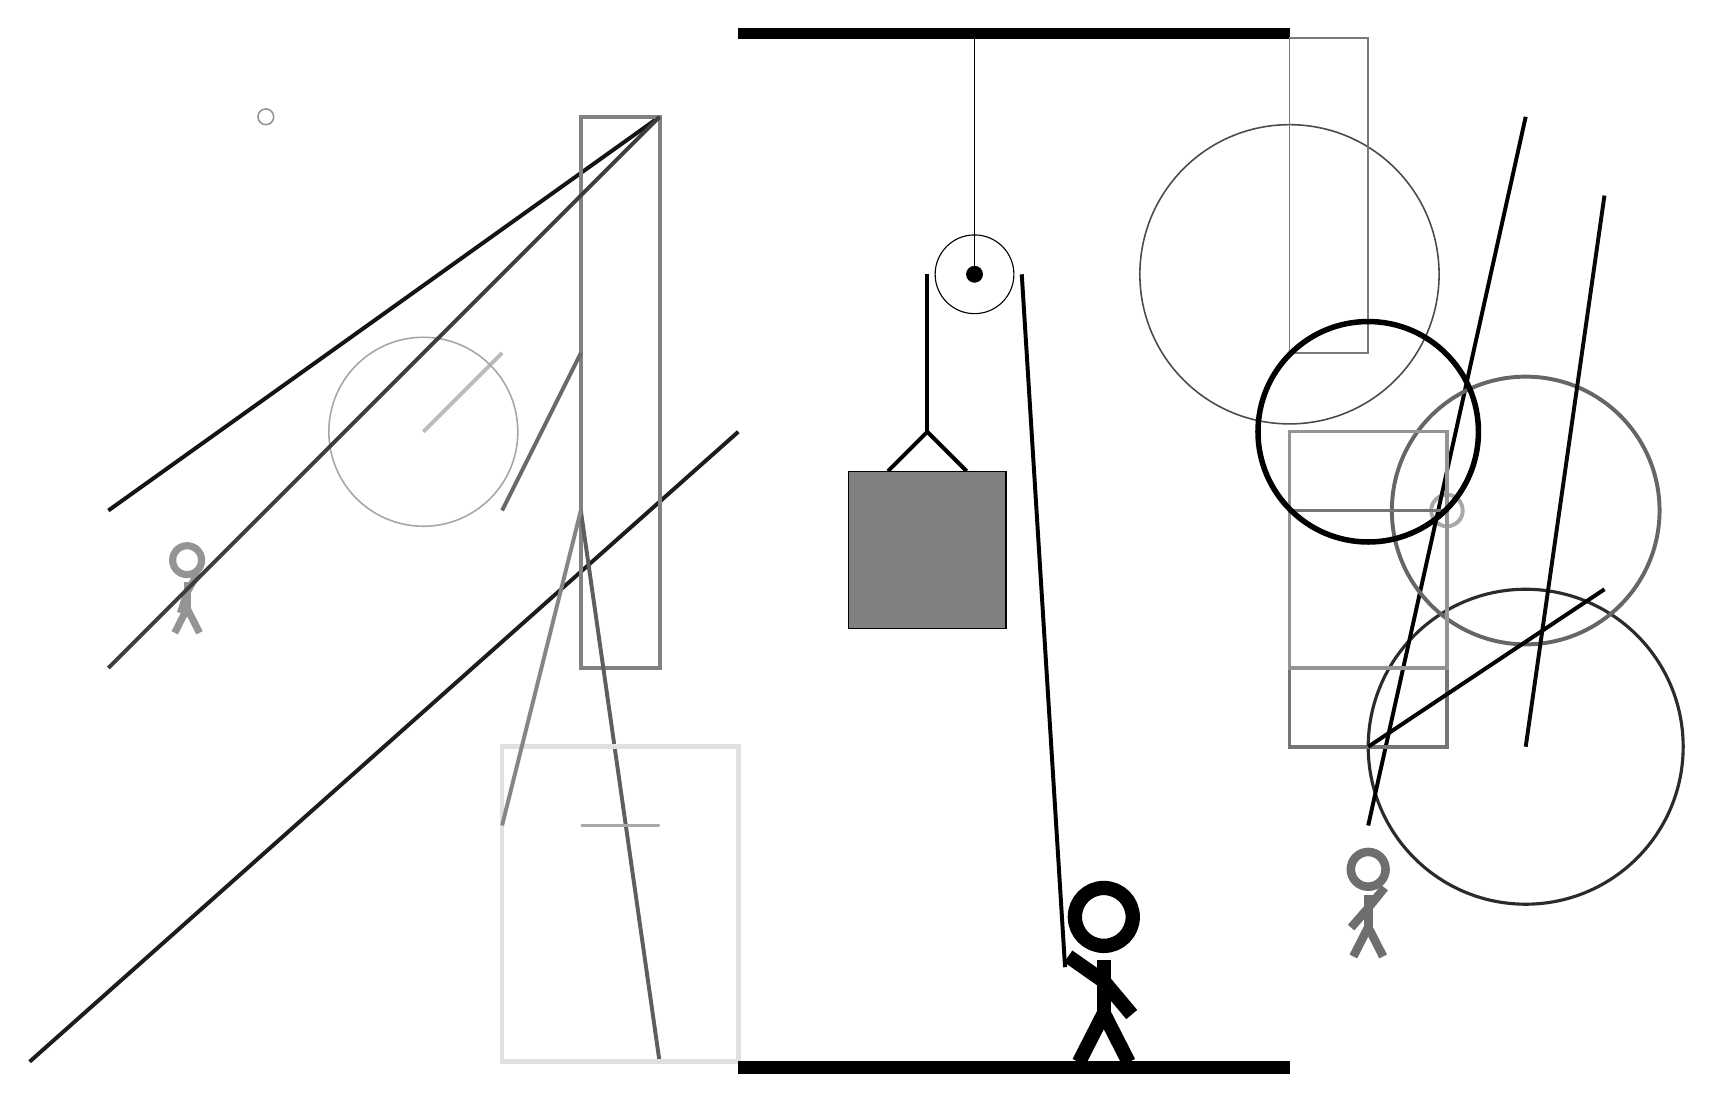
\begin{tikzpicture}
		%%%%% START %%%%%
		
		\draw[fill=black] (-2, 10) rectangle (5, 10.125);
		
		\draw (1, 7) circle (0.5);
		\draw[fill=black] (1, 7) circle (0.1);
		\draw (1, 10) -- (1, 7);
		
		\draw[line width=0.5mm] (-0.1, 4.5) -- (0.4, 5.0) -- (0.9, 4.5);
		\draw[fill=black!50] (-0.6, 4.5) rectangle (1.4, 2.5);
		
		\draw[line width=0.5mm] (0.4, 7) -- (0.4, 5.0);
		\centerarc[line width=0.5mm](1, 7)(0:180:0.6);
		\draw[line width=0.5mm](1.6, 7) -- (2.15, -1.8);
		
		\draw[line width=0.5mm, color=black!27](-5, 6) -- (-6, 5);
		
		\draw [line width=0.5mm, color=black!34](7, 4) circle (0.2);
		\draw [line width=0.4mm, color=black!83](8, 1) circle (2.0);
		\draw [line width=0.2mm, color=black!71](5, 7) circle (1.9);
		\draw[line width=0.5mm, color=black!100](6, 0) -- (8, 9);
		\draw [line width=0.2mm, color=black!35](-6, 5) circle (1.2);
		\draw[line width=0.5mm, color=black!92](-3, 9) -- (-10, 4);
		
		\draw[line width=0.5mm, color=black!89](-2, 5) -- (-11, -3);
		\draw [line width=0.5mm, color=black!60](8, 4) circle (1.7);
		
		\draw[line width=0.5mm, color=black!49] (-4, 2) rectangle (-3, 9);
		
		\node[line width=0.5mm, color=black!57] at (6, -1) {\Strichmaxerl[6][49][51]};
		
		\draw[line width=0.5mm, color=black!59](-5, 4) -- (-4, 6);
		\node[line width=0.3mm, color=black!42] at (-9, 3) {\Strichmaxerl[5][72][61]};
		\draw[line width=0.2mm, color=black!52] (6, 10) rectangle (5, 6);
		\draw[line width=0.5mm, color=black!63](-4, 4) -- (-3, -3);
		\draw[line width=0.5mm, color=black!54] (5, 1) rectangle (7, 4);
		\draw[line width=0.5mm, color=black!76](-3, 9) -- (-10, 2);
		\draw[line width=0.4mm, color=black!34] (-3, 0) rectangle (-4, 0);
		\draw[line width=0.5mm, color=black!97](9, 8) -- (8, 1);
		
		\draw[line width=0.4mm, color=black!42] (7, 5) rectangle (5, 2);
		\draw[line width=0.5mm, color=black!99](9, 3) -- (6, 1);
		\draw [line width=0.7mm, color=black!100](6, 5) circle (1.4);
		\draw[line width=0.6mm, color=black!12] (-2, -3) rectangle (-5, 1);
		\draw [line width=0.2mm, color=black!42](-8, 9) circle (0.1);
		\draw[line width=0.5mm, color=black!48](-4, 4) -- (-5, 0);
		
		\node at (2.6, -1.9) {\Strichmaxerl[10][-35][-50]};
		
		\draw[fill=black] (-2, -3) rectangle (5, -3.15);
		
		%%%%% END %%%%%
	\end{tikzpicture}
\end{document}